\documentclass{cumcmthesis}
    %\documentclass[withoutpreface,bwprint]{cumcmthesis} %去掉封面与编号页

    \title{龙门吊问题的数学建模}
    \tihao{A}            % 题号
    \baominghao{042}    % 报名号
    \schoolname{武汉大学}
    \membera{周澳}
    \memberb{傅宇千}
    \memberc{刘志豪}
    \supervisor{指导老师}
    \yearinput{2020}     % 年
    \monthinput{08}      % 月
    \dayinput{15}        % 日

\begin{document}
\maketitle
\begin{abstract}
    摘要的具体内容。
    \keywords{关键词1\quad  关键词2\quad   关键词3}
\end{abstract}
\tableofcontents
\section{问题重述}
\subsection{问题的提出}
\section{模型的假设}
\section{符号说明}
\begin{center}
    \begin{tabular}{cc}
        \hline
        \makebox[0.3\textwidth][c]{符号} & \makebox[0.4\textwidth][c]{意义} \\ \hline
        D                                & 木条宽度(cm)                   \\ \hline
    \end{tabular}
\end{center}
\section{问题分析}
如图所示建立坐标系:

\centerline{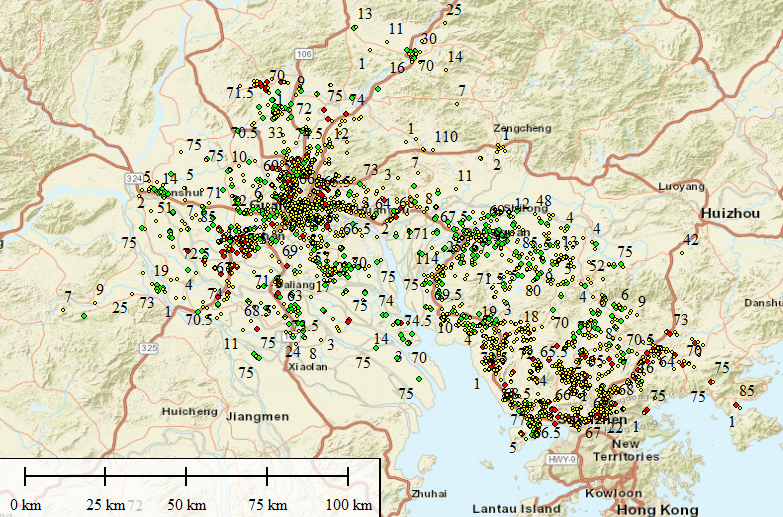
\includegraphics[width=10cm]{1.png}}
设吊车位置坐标为$x_a$,速度为$v_a$;货物的位置$(x,y)$,速度$v$,缆绳与竖直方向的角度为$\theta$(顺时针为正)

取货物为研究对象,用分析力学方法,取广义坐标$\theta$

(1)当$0~t_1$时,有如下拉格朗日函数:
$$L_{1}=\frac{m}{2}\left(l^{2} \dot{\theta}^{2}-2 a l \dot{\theta} t \cos \theta+a^{2} t^{2}\right)+m gl\cos \theta$$

代入拉格朗日方程$$\frac{d}{d t}\left(\frac{\partial L_{1}}{\partial \dot{\theta}}\right)-\frac{\partial L_1}{\partial \theta}=0$$

得到运动微分方程:$$l \ddot{\theta}+a \dot{\theta} t \sin \theta-a \cos \theta+g \sin \theta=0$$
$$\text{初始条件}\left.\theta\right|_{t=0}=0,\left.\quad \dot{\theta}\right|_{t=0}=0$$

由$\theta(t),0 \leqslant t \leqslant t_{1}$,有

$$\left\{\begin{array}{l}
        x=x_{a}-l \theta \sin \theta=\frac{a}{2} t^{2}-\operatorname{lsim} \theta \\
        v_{x}=v_{a}-l \dot{\theta} \cos \theta=a t-l \dot{\theta} \cos \theta
    \end{array}\right.$$

(2)当$t_1~t_2$时,同上可得运动微分方程:
$$\ddot{\theta}+\frac{g}{l} \sin \theta=0$$
$$\text{初始条件}\left \{\begin{array}{l}
        \left.\theta\right|_{t=t_{1}^{+}}=\left.\theta\right|_{t=t_{1}^{-}} \\
        \left.\dot{\theta}\right|_{t=t_{1}}=\left.\dot{\theta}\right|_{t=t_{1}^{-}}
    \end{array}\right.$$

此时有:$$\left\{\begin{array}{l}
        x=x_{a}-l\theta \sin \theta=\frac{a}{2} t_{1}^{2}+at_1(t-t_1)-l\sin \theta \\
        v_{x}=v_{a}-l \dot{\theta} \cos \theta=a t_{1}-l\dot{\theta }\cos \theta
    \end{array}\right.$$

(3)当$t_2~t_3$时,同(1)可得运动微分方程:
$$l \ddot{\theta}+a\left(t_{1}+t_{2}-t\right) \dot{\theta} \sin \theta+a \cos \theta+g \sin \theta=0$$
$$\text{初始条件}\left \{\begin{array}{l}
        \left.\theta\right|_{t=t_{2}^{+}}=\left.\theta\right|_{t=t_{2}^{-}} \\
        \left.\dot{\theta}\right|_{t=t_{2}}=\left.\dot{\theta}\right|_{t=t_{2}^{-}}
    \end{array}\right.$$
此时有:$$\left\{\begin{array}{l}
        v_{x}=a\left(t_{1}+t_{2}-t\right)-l \dot{ \theta} \cos \theta \\
        x=x_{2}+x_{3 a}-l\theta \sin\theta
    \end{array}\right.$$

(4)当$t_3~t_4$时,同(1)可得运动微分方程:
$$\ddot{\theta}+\frac{g}{l} \sin \theta=0$$
$$\text{初始条件}\left \{\begin{array}{l}
        \left.\theta\right|_{t=t_{3}^{+}}=\left.\theta\right|_{t=t_{3}^{-}} \\
        \left.\dot{\theta}\right|_{t=t_{3}}=\left.\dot{\theta}\right|_{t=t_{3}^{-}}
    \end{array}\right.$$
此时有:$$\left\{\begin{array}{l}
    v_{x}=a\left(t_1+t_{2}-t_{3}\right)-l \dot{\theta} \sin \theta \\
    x=x_{3}+a\left(t_{1}+t_{2}-t_{3}\right)\left(t-t_{3}\right)-l \sin \theta
    \end{array}\right.$$

最大摆角$\theta_{\max }=\max \theta(t), \quad 0 \leqslant t \leqslant t_{4}$,
取第四段匀速过程中$\theta=0$时的货物水平速度$v_{x4}$,则有
$$\begin{array}{l}
    \frac{m}{2} v_{x 4}^{2}=\frac{m}{2}(l \dot{\theta})^{2}+m g l\left(1-\cos \theta\left(t_{3}\right)\right) \\
    v_{x_{4}}^{2}=(l \dot{\theta})^{2}+2 g l\left(1-\cos \theta\left(t_{3}\right)\right)
    \end{array}$$

拉力:由$$\left\{\begin{array}{l}
    m g-T y=m a_y \\
    T_{x}=m a_{x}
    \end{array}\right.$$
可得全程拉力

\section{总结}
\begin{thebibliography}{9}%宽度9
    \bibitem{bib:one} ....
\end{thebibliography}
\begin{appendices}
    附录的内容。
\end{appendices}
\end{document}